\documentclass{exam}
\usepackage{amsmath}
\usepackage[margin=2cm]{geometry}
\usepackage[colorlinks=false]{hyperref}
\usepackage{microtype}
\usepackage{graphicx}
\usepackage{wrapfig}
\usepackage{caption}
\usepackage{subcaption}

\usepackage{pgfplots}
\usepackage{tikz}
\usetikzlibrary{arrows, positioning, calc}

\renewcommand{\d}[1]{\,\mathrm{d}#1}
\newcommand{\e}{\mathrm{e}}

% For "compressed" exam -- no vfills, pagebreaks, etc -- uncomment
% below. The actual value is unimportant; it only matters that it's
% defined. You can also call latex with something like
%
% pdflatex '\newcommand{\compressedformat}{x}\input{exam1.tex}'
%
%\newcommand{\compressedformat}{x}

%
% In the body of the exam, use \myvfill, \mynewpage, and \mycompress
% (the latter is intended to wrap tikzpicture environments, but works
% with anything.)
%
\newcommand{\mycompress}[1]{\ifdefined\compressedformat\relax\else#1\fi}
\newcommand{\myvfill}{\mycompress{\vfill}}
\newcommand{\mynewpage}{\mycompress{\newpage}}

%
% to print a big "DRAFT" on each page, uncomment below
%
%\newcommand{\draftversion}{x}
\newcommand{\drafttext}{\ifdefined\draftversion
  \begin{tikzpicture}[remember picture,overlay]
  \node [rotate=60,scale=12,color=gray!25] at (current page.center)
  {\textsf{DRAFT}};
\end{tikzpicture}
\else
  \relax
\fi}

%
% use this to add "problem continues..."
%
\newcommand{\problemcontinues}{
  \ifdefined\compressedformat
    \relax
  \else
    \runningfooter{}{\thepage\ of \numpages}{problem continues\ldots}
    \newpage
    \runningfooter{}{\thepage\ of \numpages}{}
  \fi}

%
% Change these appropriately.
%
\newcommand{\thedate}{April 9, 2015}
\newcommand{\theexam}{Homework due April 23, 2015}
\newcommand{\thecourse}{Systems, Networks, and Strategies}

\begin{document}

\pagestyle{headandfoot}
\header{\thecourse}{\theexam}{\thedate\drafttext}
\runningheadrule
\firstpageheader{\drafttext}{}{}
\firstpagefooter{}{}{}
\runningfooter{}{\thepage\ of \numpages}{}

\addpoints
\parindent 0ex

\textbf{\thecourse} \hfill  
\textbf{Name:} \makebox[6cm]{\hrulefill}

\textbf{\theexam}

\rule[1ex]{\textwidth}{.1pt}

%%% == Begin ==

\textbf{Reading:} ``Introduction to Evolution'' chapter of Wikibooks, \emph{General Biology}, \\
\url{https://en.wikibooks.org/wiki/General_Biology/Introduction_to_Evolution}.
\\*[12pt]
\question
\begin{parts} \part
What part does \textbf{variation} play in the process of natural selection?  Please answer these questions in your own words.  Very brief answers are fine.
\\*[140pt]
\part
What part does \textbf{the environment} play in natural selection?
\\*[140pt]
\part
What part does \textbf{inheritance} of traits play in natural selection?
\\*[140pt]
\part
Where does \textbf{mutation} fit into this outline of the process of natural selection?
\\*[140pt]
\end{parts}

%\mynewpage

\question
\begin{minipage}{\textwidth}
\begin{wrapfigure}[21]{r}{0.45\textwidth}
\includegraphics[width=0.4\textwidth]{Darwin's_finches_by_Gould.jpg}
\caption{\footnotesize Charles Darwin, \emph{Journal of researches into the geology and natural history of the various countries visited by H.M.S. Beagle round the world, under the command of Capt. Fitz Roy, R.N.}, second edition, 1845. Public domain, Wikimedia Commons.}
\end{wrapfigure}

\textbf{Darwin's finches.}
\\*[12pt]
The finches that Charles Darwin studied on his famous voyage to the Gal\'apagos islands have plentiful variation in their beaks. Wide and strong beaks are better at biting into the bases of local cacti, to get food from them. Long and narrow beaks are better for poking into the cactus's fruits, so different shapes are better for different years, depending on whether the cacti are producing a lot of fruit.
\\*[12pt]
Let us assume a series of dry years, so that fruit is rare.  As time passes, differences in survival and reproduction lead to changes in the population.
\end{minipage}
\\*[80pt]
\question
\begin{parts}
\part Which of the following is a plausible plot of average beak width over time?
\begin{figure}[h]
\centering
\begin{subfigure}[b]{0.35\textwidth}
\centering
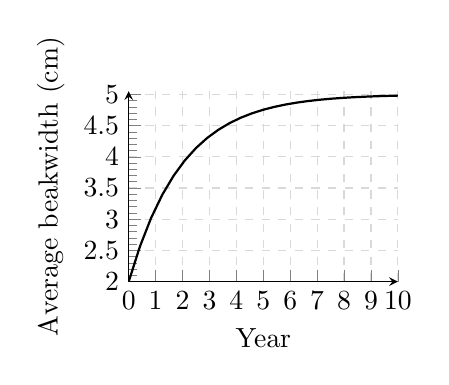
\begin{tikzpicture}
% http://martin-thoma.com/plotting-graphs-with-pgfplots-latex-and-tikz/
    \begin{axis}[
        width=5cm, height=4cm,
        axis lines=left,           % omit right and top border
        grid = major,
        grid style={dashed, gray!30},
        %xmode=log,log basis x=10,
        %ymode=log,log basis y=10,
        xmin=0,     % start the diagram at this x-coordinate
        xmax=10,   % end   the diagram at this x-coordinate
        ymin=2,     % start the diagram at this y-coordinate
        ymax=5.05,     % end   the diagram at this y-coordinate
        /pgfplots/xtick={0,1,...,10},      % draw tick and line every 1
        /pgfplots/ytick={2,2.5,...,5}, % draw tick and line every .500
        minor y tick num=4,
        %extra x ticks={23}, % add one-off ticks/lines
        %extra y ticks={0.507297},
        axis background/.style={fill=white},
        ylabel=Average beak \\width (cm),
        xlabel=Year,
        tick align=inside]

      % draw curve
      \addplot[domain=0:10, black, thick]{5 - 3*e^(-x/2)};

    \end{axis} 
\end{tikzpicture}
\caption{\mbox{}}
\end{subfigure}
\begin{subfigure}[b]{0.3\textwidth}
\centering
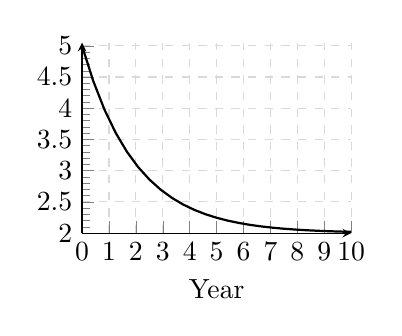
\begin{tikzpicture}
% http://martin-thoma.com/plotting-graphs-with-pgfplots-latex-and-tikz/
    \begin{axis}[
        width=5cm, height=4cm,
        axis lines=left,           % omit right and top border
        grid = major,
        grid style={dashed, gray!30},
        %xmode=log,log basis x=10,
        %ymode=log,log basis y=10,
        xmin=0,     % start the diagram at this x-coordinate
        xmax=10,   % end   the diagram at this x-coordinate
        ymin=2,     % start the diagram at this y-coordinate
        ymax=5.05,     % end   the diagram at this y-coordinate
        /pgfplots/xtick={0,1,...,10},      % draw tick and line every 1
        /pgfplots/ytick={2,2.5,...,5}, % draw tick and line every .500
        minor y tick num=4,
        %extra x ticks={23}, % add one-off ticks/lines
        %extra y ticks={0.507297},
        axis background/.style={fill=white},
        %ylabel=Average beak width (cm),
        xlabel=Year,
        tick align=inside]

      % draw curve
      \addplot[domain=0:10, black, thick]{2 + 3*e^(-x/2)};

    \end{axis} 
\end{tikzpicture}
\caption{\mbox{}}
\end{subfigure}
\begin{subfigure}[b]{0.3\textwidth}
\centering
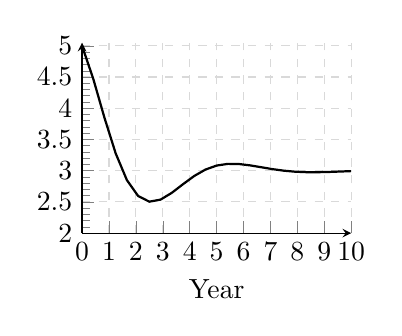
\begin{tikzpicture}
% http://martin-thoma.com/plotting-graphs-with-pgfplots-latex-and-tikz/
    \begin{axis}[
        width=5cm, height=4cm,
        axis lines=left,           % omit right and top border
        grid = major,
        grid style={dashed, gray!30},
        %xmode=log,log basis x=10,
        %ymode=log,log basis y=10,
        xmin=0,     % start the diagram at this x-coordinate
        xmax=10,   % end   the diagram at this x-coordinate
        ymin=2,     % start the diagram at this y-coordinate
        ymax=5.05,     % end   the diagram at this y-coordinate
        /pgfplots/xtick={0,1,...,10},      % draw tick and line every 1
        /pgfplots/ytick={2,2.5,...,5}, % draw tick and line every .500
        minor y tick num=4,
        %extra x ticks={23}, % add one-off ticks/lines
        %extra y ticks={0.507297},
        axis background/.style={fill=white},
        %ylabel=Average beak width (cm),
        xlabel=Year,
        tick align=inside]

      % draw curve
      \addplot[domain=0:10, black, thick]{3 + 2*e^(-x/2)*cos(60*x)};

    \end{axis} 
\end{tikzpicture}
\caption{\mbox{}}
\end{subfigure}
\end{figure}

\part 
Explain your answer briefly.
\vfill

\mynewpage
Here's a different view of the same situation, plotting the birds' ability to bite through cactus stems and ability to poke into fruit over time.
\\*[12pt]
\part Which of these is a plausible plot of the finches' changing abilities? Assume the same scenario as above, of a series of dry years?
\\*[12pt]
\emph{Notice that the left plot is ability to \emph{bite}, and the right plot is ability to \emph{poke}.}
\begin{figure}[h]
\centering
\begin{subfigure}[b]{0.4\textwidth}
\centering
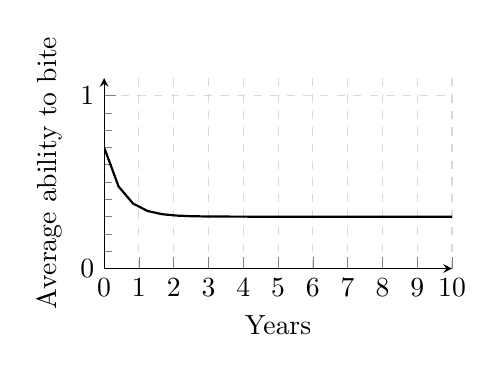
\begin{tikzpicture}
    \begin{axis}[
        width=6cm, height=4cm,
        axis lines=left,           % omit right and top border
        grid = major,
        grid style={dashed, gray!30},
        %xmode=log,log basis x=10,
        %ymode=log,log basis y=10,
        xmin=0,     % start the diagram at this x-coordinate
        xmax=10,   % end   the diagram at this x-coordinate
        ymin=0,     % start the diagram at this y-coordinate
        ymax=1.1,     % end   the diagram at this y-coordinate
        /pgfplots/xtick={0,1,...,10},      % draw tick and line every 1
        /pgfplots/ytick={0,1}, % draw tick and line every .500
        %minor x tick num=9,
        minor y tick num=9,
        %extra x ticks={23}, % add one-off ticks/lines
        %extra y ticks={0.507297},
        axis background/.style={fill=white},
        ylabel=Average ability to bite,
        xlabel=Years,
        tick align=inside]

      % draw curve
      \addplot[black, thick, domain=0:10]{0.3 + 0.4*e^(-2*x)};

    \end{axis} 
\end{tikzpicture}
\end{subfigure}
\begin{subfigure}[b]{0.3\textwidth}
\centering
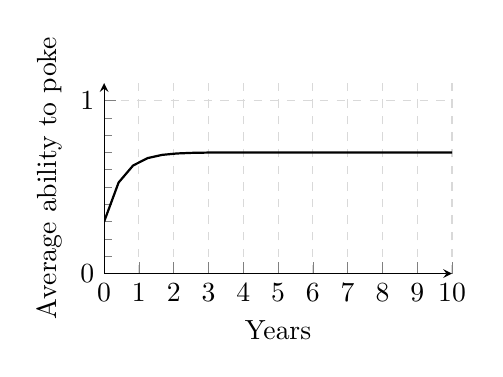
\begin{tikzpicture}
    \begin{axis}[
        width=6cm, height=4cm,
        axis lines=left,           % omit right and top border
        grid = major,
        grid style={dashed, gray!30},
        %xmode=log,log basis x=10,
        %ymode=log,log basis y=10,
        xmin=0,     % start the diagram at this x-coordinate
        xmax=10,   % end   the diagram at this x-coordinate
        ymin=0,     % start the diagram at this y-coordinate
        ymax=1.1,     % end   the diagram at this y-coordinate
        /pgfplots/xtick={0,1,...,10},      % draw tick and line every 1
        /pgfplots/ytick={0,1}, % draw tick and line every .500
        %minor x tick num=9,
        minor y tick num=9,
        %extra x ticks={23}, % add one-off ticks/lines
        %extra y ticks={0.507297},
        axis background/.style={fill=white},
        ylabel=Average ability to poke,
        xlabel=Years,
        tick align=inside]

      % draw curve
      \addplot[black, thick, domain=0:10]{0.7 - 0.4*e^(-2*x)};

    \end{axis} 
\end{tikzpicture}
\end{subfigure}

\mbox{(a)}
\end{figure}
\begin{figure}[h]
\centering
\begin{subfigure}[b]{0.4\textwidth}
\centering
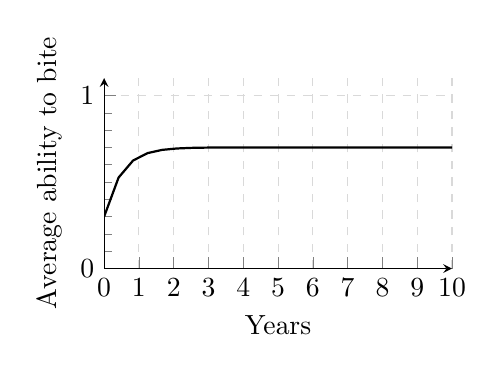
\begin{tikzpicture}
    \begin{axis}[
        width=6cm, height=4cm,
        axis lines=left,           % omit right and top border
        grid = major,
        grid style={dashed, gray!30},
        %xmode=log,log basis x=10,
        %ymode=log,log basis y=10,
        xmin=0,     % start the diagram at this x-coordinate
        xmax=10,   % end   the diagram at this x-coordinate
        ymin=0,     % start the diagram at this y-coordinate
        ymax=1.1,     % end   the diagram at this y-coordinate
        /pgfplots/xtick={0,1,...,10},      % draw tick and line every 1
        /pgfplots/ytick={0,1}, % draw tick and line every .500
        %minor x tick num=9,
        minor y tick num=9,
        %extra x ticks={23}, % add one-off ticks/lines
        %extra y ticks={0.507297},
        axis background/.style={fill=white},
        ylabel=Average ability to bite,
        xlabel=Years,
        tick align=inside]

      % draw curve
      \addplot[black, thick, domain=0:10]{0.7 - 0.4*e^(-2*x)};

    \end{axis} 
\end{tikzpicture}
\end{subfigure}
\begin{subfigure}[b]{0.3\textwidth}
\centering
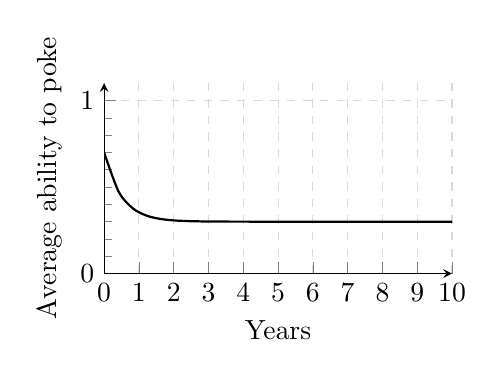
\begin{tikzpicture}
    \begin{axis}[
        width=6cm, height=4cm,
        axis lines=left,           % omit right and top border
        grid = major,
        grid style={dashed, gray!30},
        %xmode=log,log basis x=10,
        %ymode=log,log basis y=10,
        xmin=0,     % start the diagram at this x-coordinate
        xmax=10,   % end   the diagram at this x-coordinate
        ymin=0,     % start the diagram at this y-coordinate
        ymax=1.1,     % end   the diagram at this y-coordinate
        /pgfplots/xtick={0,1,...,10},      % draw tick and line every 1
        /pgfplots/ytick={0,1}, % draw tick and line every .500
        %minor x tick num=9,
        minor y tick num=9,
        %extra x ticks={23}, % add one-off ticks/lines
        %extra y ticks={0.507297},
        axis background/.style={fill=white},
        ylabel=Average ability to poke,
        xlabel=Years,
        tick align=inside]

      % draw curve
      \addplot[black, thick, smooth, domain=0:10]{0.3 + 0.4*e^(-2*x)};

    \end{axis} 
\end{tikzpicture}
\end{subfigure}

{(b)}
\end{figure}
\begin{figure}[h]
\centering
\begin{subfigure}[b]{0.4\textwidth}
\centering
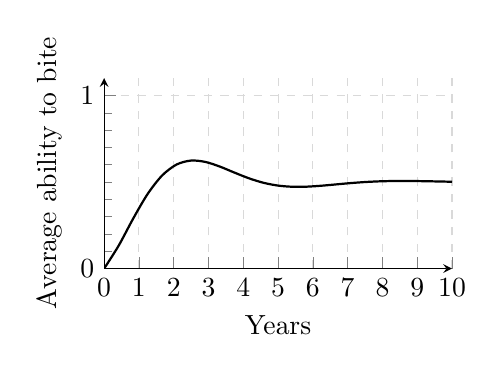
\begin{tikzpicture}
    \begin{axis}[
        width=6cm, height=4cm,
        axis lines=left,           % omit right and top border
        grid = major,
        grid style={dashed, gray!30},
        %xmode=log,log basis x=10,
        %ymode=log,log basis y=10,
        xmin=0,     % start the diagram at this x-coordinate
        xmax=10,   % end   the diagram at this x-coordinate
        ymin=0,     % start the diagram at this y-coordinate
        ymax=1.1,     % end   the diagram at this y-coordinate
        /pgfplots/xtick={0,1,...,10},      % draw tick and line every 1
        /pgfplots/ytick={0,1}, % draw tick and line every .500
        %minor x tick num=9,
        minor y tick num=9,
        %extra x ticks={23}, % add one-off ticks/lines
        %extra y ticks={0.507297},
        axis background/.style={fill=white},
        ylabel=Average ability to bite,
        xlabel=Years,
        tick align=inside]

      % draw curve
      \addplot[black, thick, smooth, domain=0:10]{0.5 - 0.5*e^(-x/2)*cos(60*x)};

    \end{axis} 
\end{tikzpicture}
\end{subfigure}
\begin{subfigure}[b]{0.3\textwidth}
\centering
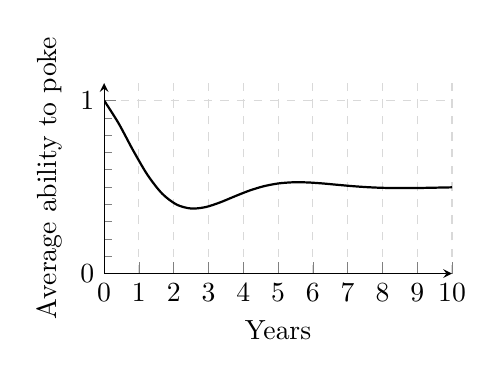
\begin{tikzpicture}
    \begin{axis}[
        width=6cm, height=4cm,
        axis lines=left,           % omit right and top border
        grid = major,
        grid style={dashed, gray!30},
        %xmode=log,log basis x=10,
        %ymode=log,log basis y=10,
        xmin=0,     % start the diagram at this x-coordinate
        xmax=10,   % end   the diagram at this x-coordinate
        ymin=0,     % start the diagram at this y-coordinate
        ymax=1.1,     % end   the diagram at this y-coordinate
        /pgfplots/xtick={0,1,...,10},      % draw tick and line every 1
        /pgfplots/ytick={0,1}, % draw tick and line every .500
        %minor x tick num=9,
        minor y tick num=9,
        %extra x ticks={23}, % add one-off ticks/lines
        %extra y ticks={0.507297},
        axis background/.style={fill=white},
        ylabel=Average ability to poke,
        xlabel=Years,
        tick align=inside]

      % draw curve
      \addplot[black, thick, smooth, domain=0:10]{0.5 + 0.5*e^(-x/2)*cos(60*x)};

    \end{axis} 
\end{tikzpicture}
\end{subfigure}

{(c)}
\end{figure}
\part Explain your answer briefly.
\vfill

\mynewpage

Here's another way to plot the same situation, using the birds' ability to bite through cactus stems and ability to poke into fruit as the two axes. So the average ability to do these things is a point somewhere in this square, and it will move from place to place as time passes.
\\*[12pt]
Since their beaks can't be good at both, the birds can't go to $(1,1)$ in the upper right corner of the square, they can only go back and forth roughly between $(0,1)$ and $(1,0)$.
\\*[12pt]
\part Which of these is a plausible plot of the finches' changing abilities? Assume the same scenario as above, of a series of dry years.
\begin{figure}[h]
\centering
\begin{subfigure}[b]{0.35\textwidth}
\centering
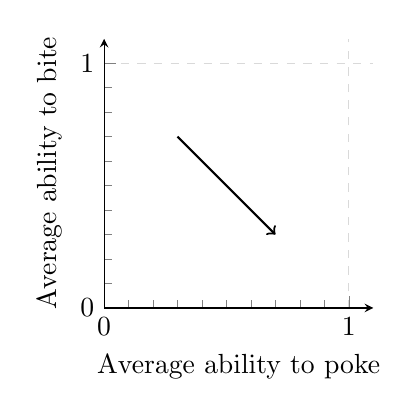
\begin{tikzpicture}
% http://martin-thoma.com/plotting-graphs-with-pgfplots-latex-and-tikz/
    \begin{axis}[
        width=5cm, height=5cm,
        axis lines=left,           % omit right and top border
        grid = major,
        grid style={dashed, gray!30},
        %xmode=log,log basis x=10,
        %ymode=log,log basis y=10,
        xmin=0,     % start the diagram at this x-coordinate
        xmax=1.1,   % end   the diagram at this x-coordinate
        ymin=0,     % start the diagram at this y-coordinate
        ymax=1.1,     % end   the diagram at this y-coordinate
        /pgfplots/xtick={0,1},      % draw tick and line every 1
        /pgfplots/ytick={0,1}, % draw tick and line every .500
        minor x tick num=9,
        minor y tick num=9,
        %extra x ticks={23}, % add one-off ticks/lines
        %extra y ticks={0.507297},
        axis background/.style={fill=white},
        ylabel=Average ability to bite,
        xlabel=Average ability to poke,
        tick align=inside]

      % draw curve
      \addplot[->, black, thick] coordinates {(0.3,0.7) (0.7,0.3)};

    \end{axis} 
\end{tikzpicture}
\caption{\mbox{}}
\end{subfigure}
\begin{subfigure}[b]{0.3\textwidth}
\centering
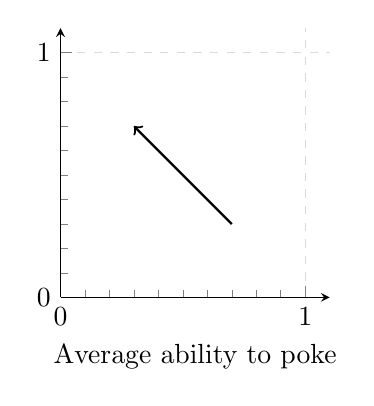
\begin{tikzpicture}
% http://martin-thoma.com/plotting-graphs-with-pgfplots-latex-and-tikz/
    \begin{axis}[
        width=5cm, height=5cm,
        axis lines=left,           % omit right and top border
        grid = major,
        grid style={dashed, gray!30},
        %xmode=log,log basis x=10,
        %ymode=log,log basis y=10,
        xmin=0,     % start the diagram at this x-coordinate
        xmax=1.1,   % end   the diagram at this x-coordinate
        ymin=0,     % start the diagram at this y-coordinate
        ymax=1.1,     % end   the diagram at this y-coordinate
        /pgfplots/xtick={0,1},      % draw tick and line every 1
        /pgfplots/ytick={0,1}, % draw tick and line every .500
        minor x tick num=9,
        minor y tick num=9,
        %extra x ticks={23}, % add one-off ticks/lines
        %extra y ticks={0.507297},
        axis background/.style={fill=white},
        %ylabel=Average ability to bite,
        xlabel=Average ability to poke,
        tick align=inside]

      % draw curve
      \addplot[->, black, thick] coordinates {(0.7,0.3) (0.3,0.7)};

    \end{axis} 
\end{tikzpicture}
\caption{\mbox{}}
\end{subfigure}
\end{figure}
\part Explain your answer briefly.
\vfill

\mynewpage

Now suppose that after the above scenario happens, after a thousand years, a rare mutation arises that gives a bird the ability to use a stick as a tool to poke into cactus fruit, so that they can do it while having thick beaks.
\\*[12pt]
\part Which of these is a plausible plot of what happens?
\begin{figure}[h]
\centering
\begin{subfigure}[b]{0.35\textwidth}
\centering
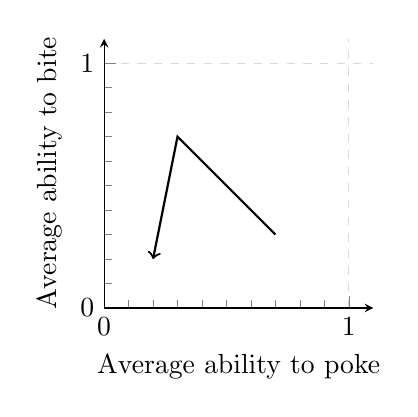
\begin{tikzpicture}
% http://martin-thoma.com/plotting-graphs-with-pgfplots-latex-and-tikz/
    \begin{axis}[
        width=5cm, height=5cm,
        axis lines=left,           % omit right and top border
        grid = major,
        grid style={dashed, gray!30},
        %xmode=log,log basis x=10,
        %ymode=log,log basis y=10,
        xmin=0,     % start the diagram at this x-coordinate
        xmax=1.1,   % end   the diagram at this x-coordinate
        ymin=0,     % start the diagram at this y-coordinate
        ymax=1.1,     % end   the diagram at this y-coordinate
        /pgfplots/xtick={0,1},      % draw tick and line every 1
        /pgfplots/ytick={0,1}, % draw tick and line every .500
        minor x tick num=9,
        minor y tick num=9,
        %extra x ticks={23}, % add one-off ticks/lines
        %extra y ticks={0.507297},
        axis background/.style={fill=white},
        ylabel=Average ability to bite,
        xlabel=Average ability to poke,
        tick align=inside]

      % draw curve
      \addplot[->, black, thick] coordinates {(0.7,0.3) (0.3,0.7) (0.2,0.2)};

    \end{axis} 
\end{tikzpicture}
\caption{\mbox{}}
\end{subfigure}
\begin{subfigure}[b]{0.3\textwidth}
\centering
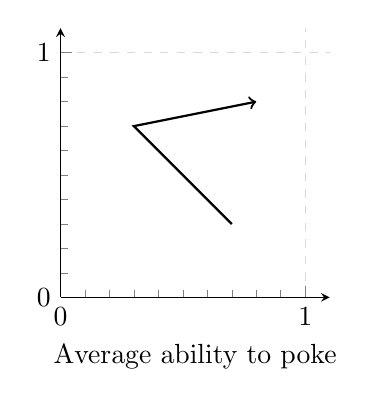
\begin{tikzpicture}
% http://martin-thoma.com/plotting-graphs-with-pgfplots-latex-and-tikz/
    \begin{axis}[
        width=5cm, height=5cm,
        axis lines=left,           % omit right and top border
        grid = major,
        grid style={dashed, gray!30},
        %xmode=log,log basis x=10,
        %ymode=log,log basis y=10,
        xmin=0,     % start the diagram at this x-coordinate
        xmax=1.1,   % end   the diagram at this x-coordinate
        ymin=0,     % start the diagram at this y-coordinate
        ymax=1.1,     % end   the diagram at this y-coordinate
        /pgfplots/xtick={0,1},      % draw tick and line every 1
        /pgfplots/ytick={0,1}, % draw tick and line every .500
        minor x tick num=9,
        minor y tick num=9,
        %extra x ticks={23}, % add one-off ticks/lines
        %extra y ticks={0.507297},
        axis background/.style={fill=white},
        %ylabel=Average ability to bite,
        xlabel=Average ability to poke,
        tick align=inside]

      % draw curve
      \addplot[->, black, thick] coordinates {(0.7,0.3) (0.3,0.7) (0.8,0.8)};

    \end{axis} 
\end{tikzpicture}
\caption{\mbox{}}
\end{subfigure}
\begin{subfigure}[b]{0.3\textwidth}
\centering
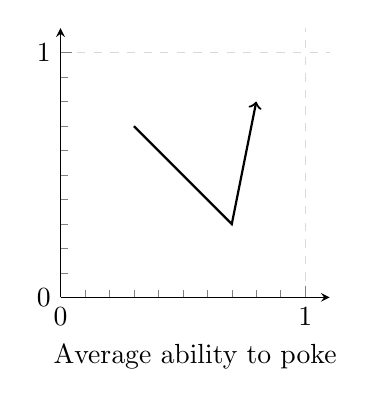
\begin{tikzpicture}
% http://martin-thoma.com/plotting-graphs-with-pgfplots-latex-and-tikz/
    \begin{axis}[
        width=5cm, height=5cm,
        axis lines=left,           % omit right and top border
        grid = major,
        grid style={dashed, gray!30},
        %xmode=log,log basis x=10,
        %ymode=log,log basis y=10,
        xmin=0,     % start the diagram at this x-coordinate
        xmax=1.1,   % end   the diagram at this x-coordinate
        ymin=0,     % start the diagram at this y-coordinate
        ymax=1.1,     % end   the diagram at this y-coordinate
        /pgfplots/xtick={0,1},      % draw tick and line every 1
        /pgfplots/ytick={0,1}, % draw tick and line every .500
        minor x tick num=9,
        minor y tick num=9,
        %extra x ticks={23}, % add one-off ticks/lines
        %extra y ticks={0.507297},
        axis background/.style={fill=white},
        %ylabel=Average ability to bite,
        xlabel=Average ability to poke,
        tick align=inside]

      % draw curve
      \addplot[->, black, thick] coordinates {(0.3,0.7) (0.7,0.3) (0.8,0.8)};

    \end{axis} 
\end{tikzpicture}
\caption{\mbox{}}
\end{subfigure}
\end{figure}
\part Explain your answer briefly.
\vfill

\end{parts}

\end{document}
